\chapter{RF Refactoring延伸功能之實作}
\indent
本章將對第三章所敘述之設計進行實作,其將針對RF Refactoring的兩個子系統進行擴充,分別為重構功能子系統及外掛程式子系統,後續小節將針對擴充之系統架構與子系統進行介紹。

\section{系統架構}\label{s4.1}
\indent
圖\ref{f4.1}為RF Refactoring延伸功能實作的系統架構圖,粗框元件代表擴充後的子系統,下列為各元件之介紹:

\begin{itemize}

\item\textbf{Eclipse:}
除基礎核心外皆為外掛程式之開源整合式開發環境

\item\textbf{Expanded Refactoring Plugin:}
擴充後提供使用者進行重構之Eclipse外掛程式

\item\textbf{Expanded Refactoring Function:}
以Python實作之擴充後外掛程式

\item\textbf{Robot Framework Parsing API:}
Robot Framework提供解析測試檔案的應用程式介面

\item\textbf{Test Script:}
測試腳本及測試資源

\end{itemize}

\indent
黑粗框元件為本論文主要之元件,其中Expanded Refactoring Plugin於Eclipse上針對Robot Framework測試檔案提供使用者更加多元的重構功能。使用者利用Expanded Refactoring Plugin中的使用者介面進行重構時,其會透過Jython函式庫呼叫Expanded Refactoring Function進行重構。重構功能將新增兩種,分別為抽取重複步驟成為新關鍵字及移動關鍵字宣告,而其流程將如\ref{s3.2}節及\ref{s3.3}節中所敘述,透過自動搜尋所需的資訊後,於Eclipse上的視圖及視窗提供使用者進行選取,並自動確保關鍵字所需測試資源都有確實被引入,不會導致未知關鍵字之錯誤。

\begin{figure}[H]
    \centering
    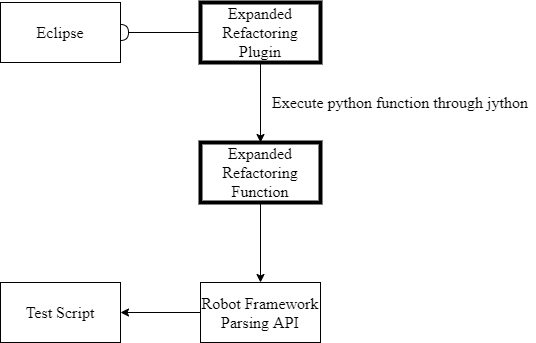
\includegraphics[width=1.0\textwidth]{picture/ch4/System_structure.png}
    \caption{RF Refactoring延伸功能實作之系統架構圖}
    \label{f4.1}
\end{figure}
\newpage

\section{重構功能之擴充}\label{s4.2}
\indent
圖\ref{f4.2}為擴充的重構功能子系統類別圖,下列為圖中各類別之介紹:

\begin{itemize}

\item\textbf{NodeVisitor:}
位於AST套件中的類別,其提供針對抽象語法樹的拜訪,並且提供部分方法可被覆寫,可依照需求做調整。

\item\textbf{NodeTransformer:}
位於AST套件中的類別,與NodeVisitor很像,但額外提供了對於抽象語法樹的修改,可依照需求修改語法樹的內容。

\item\textbf{TestModelBuilder:}
用於解析測試專案中的測試檔案,且將解析後的AST模型提供給其他類別使用。

\item\textbf{LineKeywordsHelper:}
針對使用者選取出的測試步驟,進行資料處理,例如:取得未定義於測試步驟中的變數、將測試步驟字串化以提供顯示等等。

\item\textbf{KeywordCreator:}
繼承NodeTransformer類別,主要用於建立新關鍵字中的測試步驟、創立一個新關鍵字及以新關鍵字取代重複步驟。

\item\textbf{KeywordMoveHelper:}
繼承NodeTransformer類別,主要用於移動關鍵字宣告、移動關鍵字所需測試資源。

\item\textbf{FileChecker:}
繼承NodeVisitor類別,主要用於搜尋未引入關鍵字所需測試資源的測試檔案、搜尋使用特定關鍵字宣告的測試檔案及搜尋含有重複步驟的測試檔案等等。

\item\textbf{KeywordFinder:}
繼承NodeVisitor類別,主要用於搜尋關鍵字宣告、搜尋被使用的關鍵字。

\item\textbf{NewRefactoringFacade:}
負責提供新重構功能給Eclipse外掛程式使用的類別,其提供解析測試專案、創立新關鍵字、搜尋所有重複步驟、移動關鍵字宣告、搜尋未引入所需測試資源的測試檔案等等功能。

\end{itemize}

\begin{figure}[H]
	\centering
    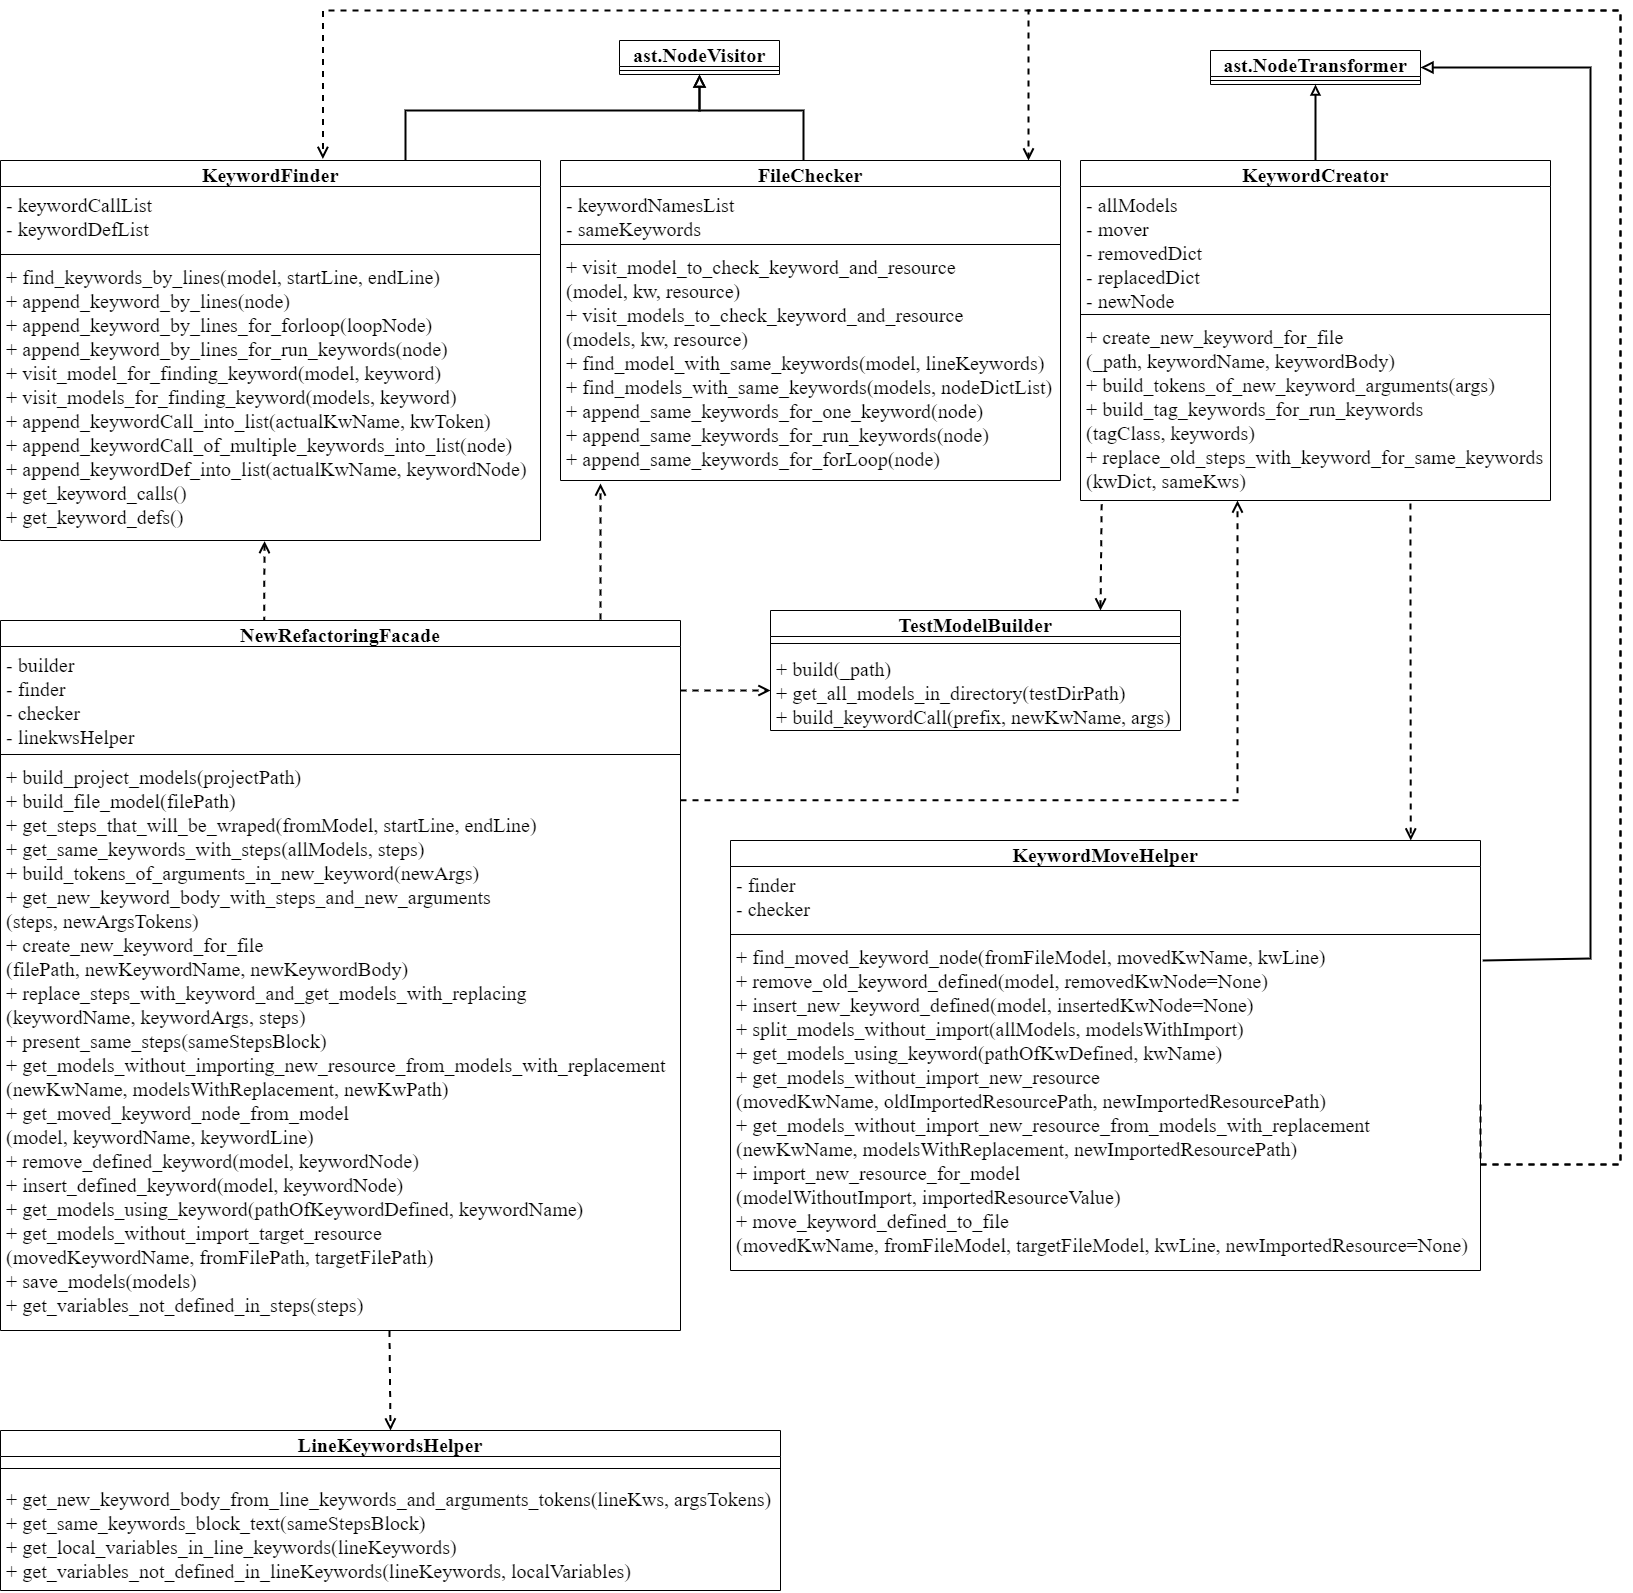
\includegraphics[width=1.0\textwidth]{picture/ch4/Feature_class.png}
    \caption{重構功能擴充之類別圖}
    \label{f4.2}
\end{figure}

\indent
在此類別圖中,NewRefactoringFacade會實作各種重構介面,提供後續外掛程式能夠方便地使用擴充之重構功能,其將透過KeywordFinder及FileChecker尋找符合特定條件的關鍵字或測試檔案,以達到尋找重複步驟和使用特定關鍵字之測試檔案的目的,並且使用TestModelBuilder解析測試檔案來提供所有AST模型。而為了達成創建關鍵字以及移動關鍵字宣告之目的,將會透過KeywordCreator及KeywordMoveHelper實作相關之功能。下列小節將針對各功能之實作進行說明。

\section{預先解析測試專案之實作}
\indent
在Robot Framework中,測試檔案分為測試套件及測試資源兩種,本論文利用Robot Framework Parsing API套件之函式解析測試套件及測試資源,其參數都是檔案路徑。圖\ref{f4.3}為預先解析測試專案之循序圖,取得測試專案的路徑後,將其傳入TestModelBuilder類別之函式,其將會透過遞迴方式搜尋是否有測試套件及測試資源,如搜尋到的檔案為測試套件,則利用api套件中的get model取得其AST模型,反之則利用get resource model,進而解析出專案下全部的測試套件及測試資源,提供其他實作功能使用。

\begin{figure}[H]
	\centering
    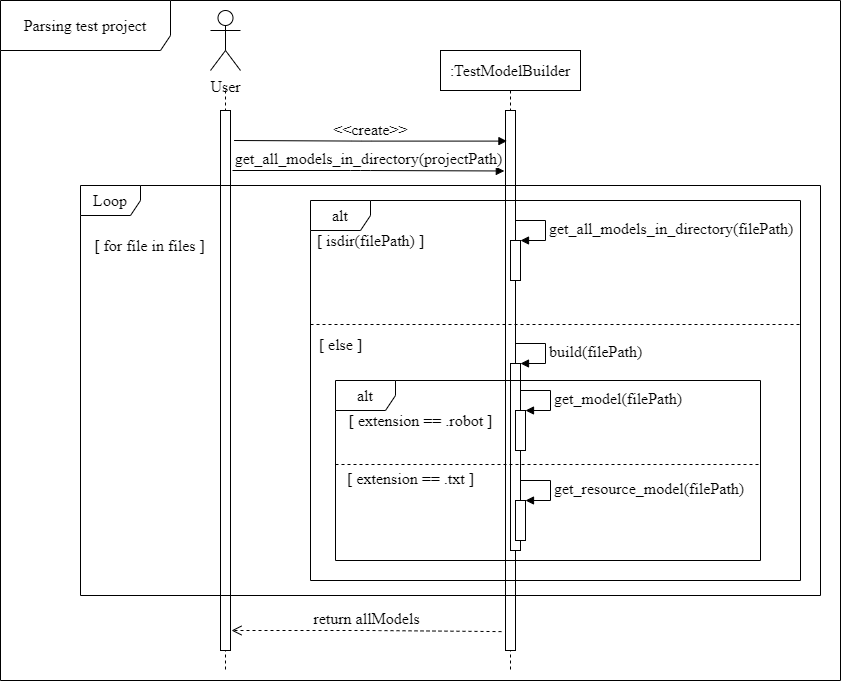
\includegraphics[width=1.0\textwidth]{picture/ch4/sequenceDiagram/Parsing_test_project_sequence_diagram.png}
    \caption{預先解析測試專案之循序圖}
    \label{f4.3}
\end{figure}

\section{抽取重複步驟成為新關鍵字之實作}
本論文將依照\ref{s3.2}節所敘述之流程進行實作,透過KeywordFinder、FileChecker及KeywordCreator等類別完成下列各功能,進而達到抽取重複步驟成為新關鍵字之目的。

\subsection{創立新關鍵字}\label{s4.4.1}
%\indent
%如\ref{s3.2.2}節所敘述,本論文將依照所決定之步驟作為新關鍵字中的測試步驟,進而創立新關鍵字,圖\ref{f4.4}為此功能之循序圖,每個類別將會執行其負責的功能,進而完成此主要功能。根據AST模型及步驟所在的行數區間呼叫KeywordFinder類別中的函式,其可利用抽象語法樹各個節點,搜尋其所需的測試步驟,針對每個被呼叫的關鍵字將會比對其是否位於要求的行數區間,藉此取得所需的測試步驟。
%
%\indent
%在所需的測試步驟中,透過LineKeywordsHelper類別中的函式,針對每個關鍵字的參數進行比對,當其含有變數所需的三種型態構造時,則將其加入搜尋結果,例如:\$\{Variable\}、@\{List\}及\&\{Dictionary\},後續則會得出測試步驟中的所有變數。在取得所有變數後,必須在測試步驟中搜尋是否有任何指派變數數值的關鍵字,如果有變數遭指派數值,則將其視為區域變數,其餘未被指派者皆得被認定為未宣告之變數,當未宣告變數數量大於零時,將透過KeywordCreator類別將其自動作為新關鍵字之參數,反之新關鍵字不會自動產生任何參數。此時KeywordCreator類別中的函式將依照指定的檔案路徑、新關鍵字名稱及經過處理的新關鍵字內容,完成新關鍵字之創立並將被修改的AST模型透過儲存函式回存至檔案系統中。
\indent
如\ref{s3.2.2}節所敘述,本論文將依照所決定之步驟作為新關鍵字中的測試步驟,進而創立新關鍵字,圖\ref{f4.4}為此功能之循序圖,根據AST模型及步驟所在的行數區間呼叫KeywordFinder類別中的函式,即可取得其指定的測試步驟。透過LineKeywordsHelper類別之函式,在測試步驟中搜尋是否有變數之宣告,如有則將其視為區域變數,其餘皆認定為未宣告之變數。當未宣告變數數量大於零時,將透過KeywordCreator類別將其作為新關鍵字之參數,後續將依照指定的檔案路徑、新關鍵字名稱及經過處理的新關鍵字內容,完成新關鍵字之創立並將被修改的AST模型透過儲存函式回存至檔案系統中。

\begin{figure}[H]
	\centering
    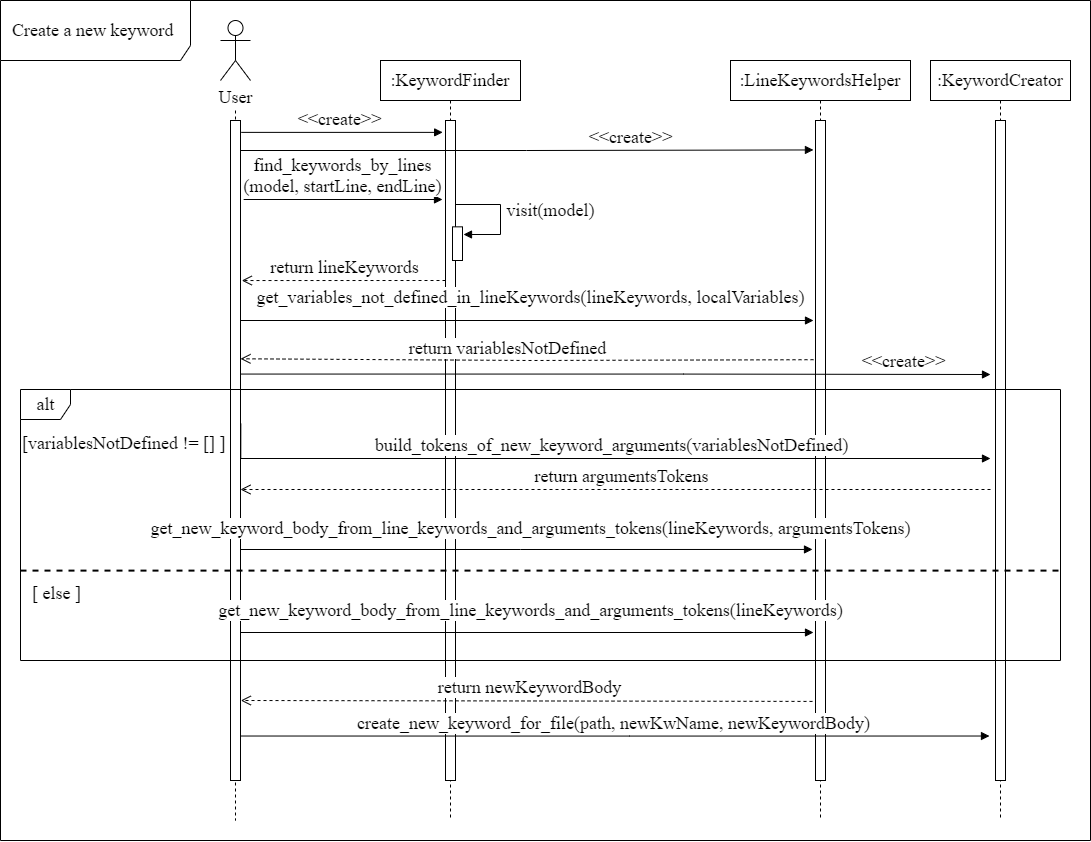
\includegraphics[width=1.0\textwidth]{picture/ch4/sequenceDiagram/Create_new_keyword_sequence_diagram.png}
    \caption{創立新關鍵字之循序圖}
    \label{f4.4}
\end{figure}
\newpage

\subsection{搜尋所有相關重複步驟並取代}\label{s4.4.2}
%\indent
%根據\ref{s3.2.3}節所敘述之流程,本論文將\ref{s4.4.1}節所決定之測試步驟作為重複步驟判定之依據,進而得出專案中含有重複步驟之測試檔案,後續將選擇的重複步驟使用新關鍵字進行取代。圖\ref{f4.5}為搜尋所有相關重複步驟並取代之循序圖,FileChecker類別中的函式將拜訪提前被解析完成的所有AST模型,從每個AST模型中拜訪關鍵字節點,例如:測試腳本中的關鍵字、關鍵字宣告中的被呼叫關鍵字及For Loop迴圈中的關鍵字等等。藉由判定多個步驟與依據步驟的排序、參數數量和關鍵字名稱是否相同,確認其是否為重複之步驟,如是則將其當下檔案資訊、抽象語法樹的節點、步驟資訊透過Dictionary儲存下來,並將其存入搜尋結果中,最後將會得到重複步驟之清單。
%
%\indent
%重複步驟清單經過選擇後,需要以新關鍵字進行取代的重複步驟,將會被傳入KeywordCreator類別中的函式進行取代。首先會判定步驟是否為重複步驟內容之最後一步,若不是,將會拜訪步驟所屬檔案中的每個節點,找出該步驟之節點將其從AST模型中移除,並將被修改的AST模型更新至全部AST模型中;反之步驟為重複步驟內容之最後一步時,則會找出該步驟之節點後,利用新關鍵字之資訊取代該步驟之節點,同樣將修改後的AST模型更新回全部AST模型中,針對每組重複步驟進行上述處理,以此完成該功能。
\indent
根據\ref{s3.2.3}節之流程,將\ref{s4.4.1}節所決定之測試步驟作為重複步驟判定之依據,得出專案中含有重複步驟之測試檔案,最後將選擇的重複步驟使用新關鍵字進行取代。圖\ref{f4.5}為搜尋所有相關重複步驟並取代之循序圖,FileChecker類別將拜訪所有AST模型,藉由判定多個步驟與依據步驟的排序、參數數量和關鍵字名稱是否相同,確認其是否為重複步驟,如是則存入搜尋結果中,最後得到重複步驟清單。重複步驟清單經過選擇後,將會透過KeywordCreator類別進行取代,首先判斷步驟是否為重複步驟之最後一步,若不是,將會從AST模型中移除;反之則以新關鍵字取代,每組重複步驟皆進行上述處理,最後完成該功能。

\begin{figure}[H]
	\centering
    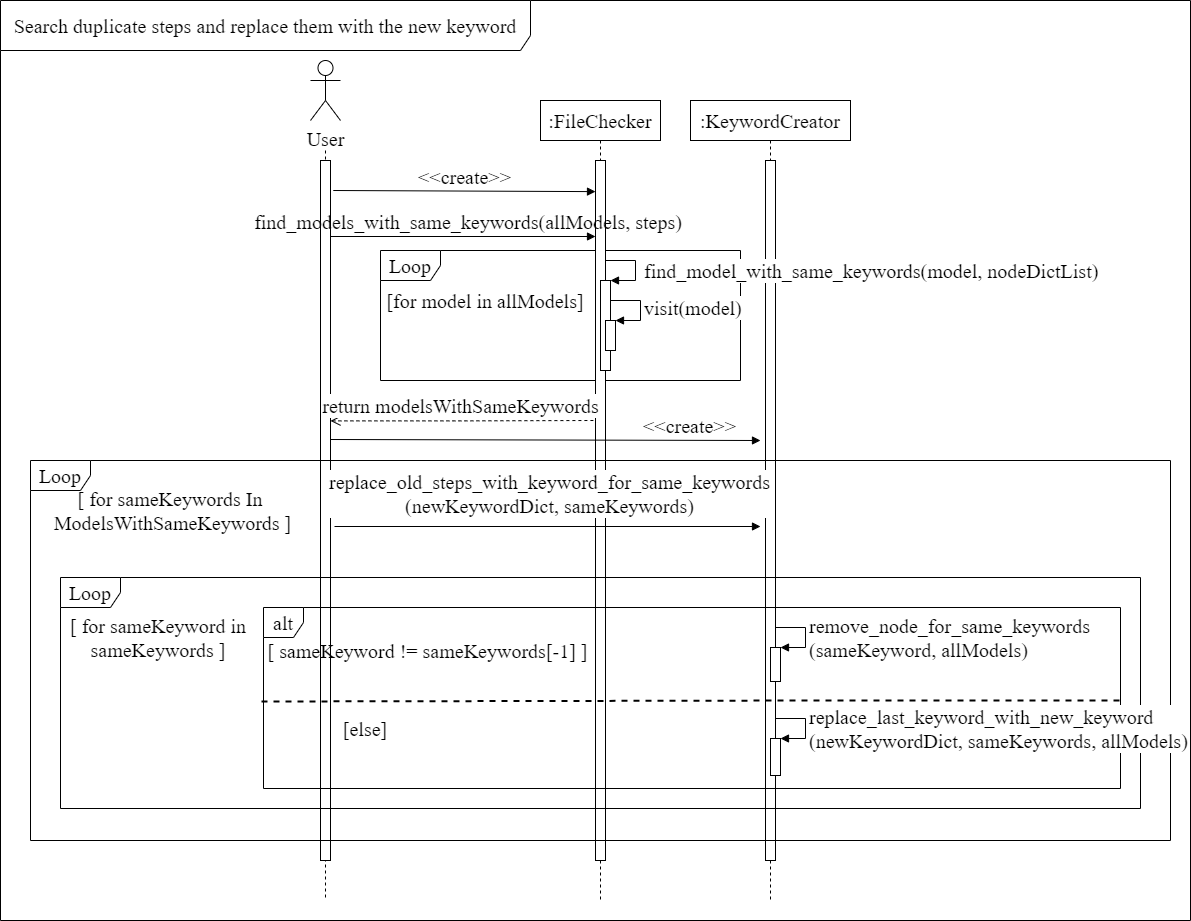
\includegraphics[width=1.0\textwidth]{picture/ch4/sequenceDiagram/Search_duplicate_steps_and_replace_sequence_diagram.png}
    \caption{搜尋所有相關重複步驟並取代之循序圖}
    \label{f4.5}
\end{figure}

\subsection{搜尋未引入所需測試資源的測試檔案並自動引入}
%\indent
%依據\ref{s3.2.4}節敘述之流程,本論文將保留\ref{s4.4.2}節使用新關鍵字之AST模型,不需再從全部AST模型中搜尋,且修正其中未引入新關鍵字所需測試資源的測試檔案。圖\ref{f4.6}為搜尋未引入所需測試資源的測試檔案並自動引入之循序圖,將保留的AST模型及所需測試資源的路徑傳入KeywordMoveHelper類別之函式,其將透過FileChecker類別之函式拜訪每個AST模型的測試資源節點,比對每個AST模型所引入的測試資源是否與新關鍵字所需之名稱吻合,一旦發現AST模型符合條件時,則將其列入排除清單,最後與所有AST模型比對得出需要修正之測試檔案。
%
%\indent
%所有需要引入新測試資源的測試檔案,將透過KeywordMoveHelper類別之函式,拜訪其中的Settings節點,並為其引入所需的測試資源,最後將修正後的AST模型進行儲存並更新回全部AST模型中,確保後續進行其他重構時,檔案內容皆為正確。
\indent
依據\ref{s3.2.4}之流程,保留\ref{s4.4.2}節使用新關鍵字之AST模型,且修正其中未引入新關鍵字所需測試資源的測試檔案。圖\ref{f4.6}為搜尋未引入所需測試資源的測試檔案並自動引入之循序圖,KeywordMoveHelper類別之函式將透過FileChecker類別,比對每個AST模型所引入的測試資源是否含有新關鍵字所需測試資源,最後與所有AST模型比對得出需要修正之測試檔案。需要修正的測試檔案,將透過KeywordMoveHelper類別之函式,為其引入所需的測試資源,最後更新修正後的AST模型至全部AST模型中,確保後續進行其他重構時,檔案內容皆為正確。

\begin{figure}[H]
	\centering
    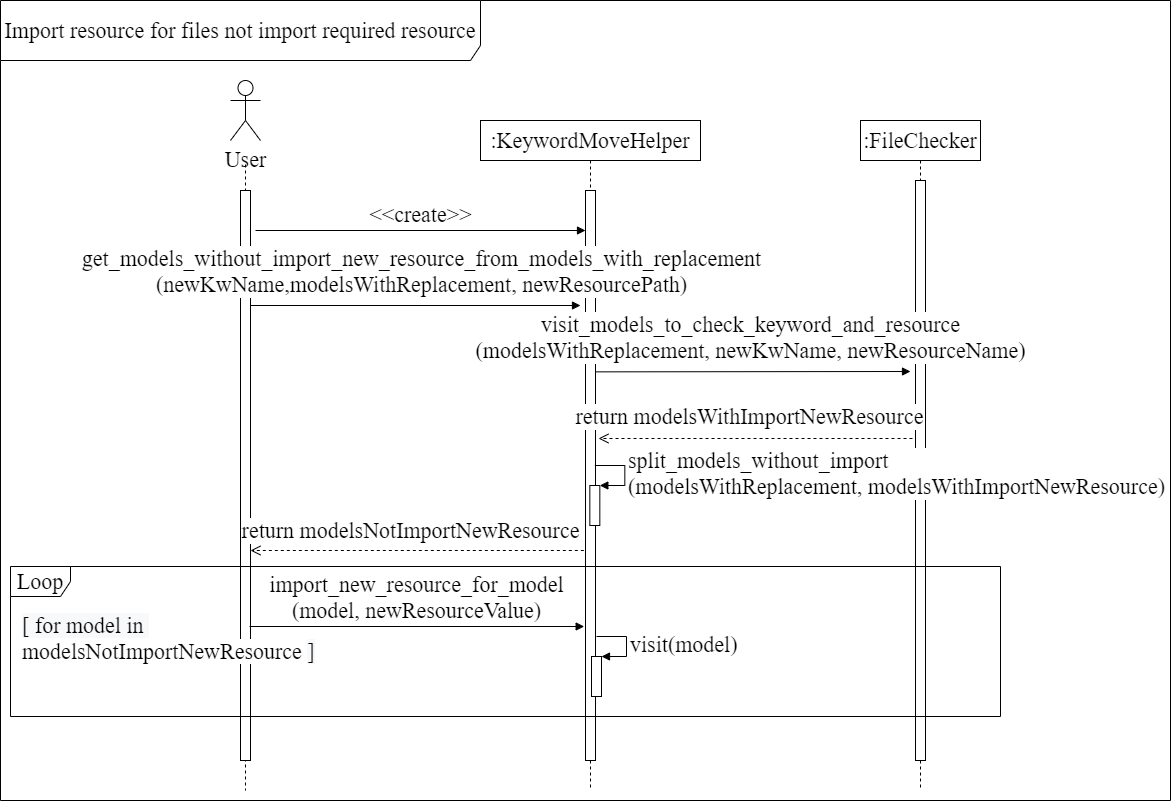
\includegraphics[width=1.0\textwidth]{picture/ch4/sequenceDiagram/Import_resource_for_files_not_import_required_resource_sequence_diagram.png}
    \caption{搜尋未引入所需測試資源的測試檔案並自動引入之循序圖}
    \label{f4.6}
\end{figure}

\section{移動關鍵字宣告之實作}
\indent
本論文將依照\ref{s3.3}節所敘述之流程進行實作,透過KeywordFinder、FileChecker及KeywordMoveHelper等類別完成下列各功能,進而達到移動關鍵字宣告之目的。

\subsection{移動關鍵字宣告}
%\indent
%藉由\ref{s3.3.2}節所敘述之流程,本論文將會把需被移動之關鍵字宣告從其所屬檔案中移除,並將其完整複製至指定檔案的關鍵字列表中,以此完成此功能。圖\ref{f4.7}為移動關鍵字宣告之循序圖,透過KeywordFinder類別之函式,拜訪關鍵字宣告所屬檔案之AST模型的所有關鍵字宣告節點,比對其名稱是否與所要移動的關鍵字名稱符合,如是則將其加入搜尋結果,最後得出符合條件之關鍵字宣告清單。
%
%\indent
%在符合條件之關鍵字清單中,檢查其數量是否只有一個,如不是則檔案中可能已存在關鍵字重複宣告之錯誤或此檔案中並無此關鍵字宣告,因此必須中止此重構;反之將會以唯一的關鍵字宣告進行移動。利用KeywordMoveHelper類別之函式,拜訪所屬檔案之AST模型的所有關鍵字宣告,並將欲移動之關鍵字宣告節點從AST模型中移除,後續則拜訪移動目的地之AST模型的Keywords節點,將關鍵字宣告移動到此檔案中,最後將修改的AST模型進行儲存並更新至全部AST模型之中,確保最終檔案內容之正確。
\indent
藉由\ref{s3.3.2}節之流程,將會把需被移動之關鍵字宣告從其所屬檔案中移除,並將其完整複製至指定檔案的關鍵字列表中。圖\ref{f4.7}為移動關鍵字宣告之循序圖,透過KeywordFinder類別之函式,比對關鍵字宣告名稱是否與所要移動的關鍵字名稱符合,如是則將其加入搜尋結果,最後得出關鍵字宣告清單。在關鍵字宣告清單中,如果數量只有一個則將其移動;反之則檔案中可能已存在關鍵字重複宣告之錯誤或此檔案中並無此關鍵字宣告,因此必須中止此重構。最後利用KeywordMoveHelper類別之函式,將欲移動之關鍵字宣告從AST模型中移除,並將其移動到目標檔案中。

\begin{figure}[H]
	\centering
    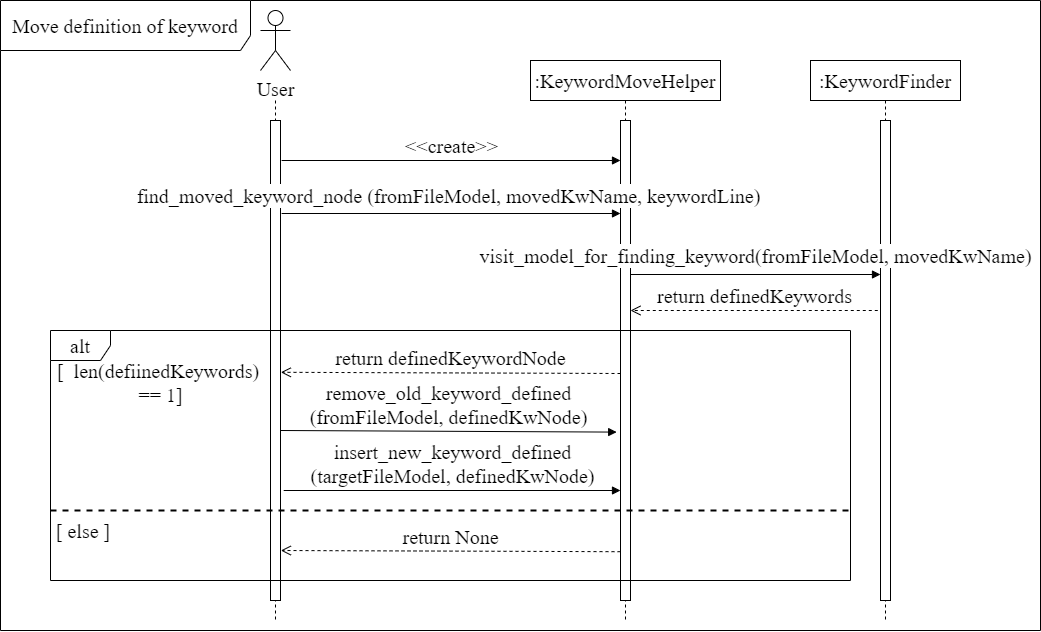
\includegraphics[width=0.93\textwidth]{picture/ch4/sequenceDiagram/Move_definition_of_keyword_sequence_diagram.png}
    \caption{移動關鍵字之循序圖}
    \label{f4.7}
\end{figure}

\subsection{搜尋使用被移動關鍵字但未引入所需測試資源的測試檔案並自動引入}
%\indent
%根據\ref{s3.3.3}節所敘述之流程,本論文將從所有的AST模型中,搜尋有使用被移動關鍵字之測試檔案,並檢測其是否有引入被移動關鍵字所需之新測試資源,如未引入則自動為其修正。圖\ref{f4.8}為搜尋使用被移動關鍵字但未引入所需測試資源的測試檔案並自動引入之循序圖,透過FileChecker類別之函式,其將會拜訪所有AST模型中每個關鍵字節點,比對其名稱是否與被移動關鍵字宣告之名稱相同,並拜訪每個測試資源節點,驗證其是否有引入原先所需測試資源,如果兩種條件皆符合,即將其AST模型列入搜尋結果,以此取得使用被移動關鍵字之測試檔案。
%
%\indent
%KeywordMoveHelper類別將藉由FileChecker類別之函式,拜訪上述已取得之AST模型,從每個測試資源節點中,驗證其是否有引入所需之新測試資源,如是則列入搜尋結果,最後與全部AST模型進行反向排除,得到未引入所需新測試資源的全部測試檔案。透過KeywordMoveHelper類別之函式,拜訪每個測試檔案之AST模型,在其中的Settings節點引入所需的測試資源,最後將修正後的AST模型進行儲存並更新回全部AST模型中。
\indent
根據\ref{s3.3.3}節之流程,搜尋使用被移動關鍵字之測試檔案,並修正其中未引入所需測試資源的測試檔案。圖\ref{f4.8}為搜尋使用被移動關鍵字但未引入所需測試資源的測試檔案並自動引入之循序圖,透過FileChecker類別之函式,於檔案中比對關鍵字名稱與被移動關鍵字宣告之名稱是否相同,並驗證其是否有引入原先所需測試資源,如果兩種條件皆符合,則將其列入搜尋結果,以此取得使用被移動關鍵字之測試檔案。最後KeywordMoveHelper類別將藉由FileChecker類別之函式,得出有引入所需測試資源之AST模型,並與全部AST模型比對得到未引入所需測試資源的測試檔案,且為其引入所需測試資源	。

\begin{figure}[H]
	\centering
    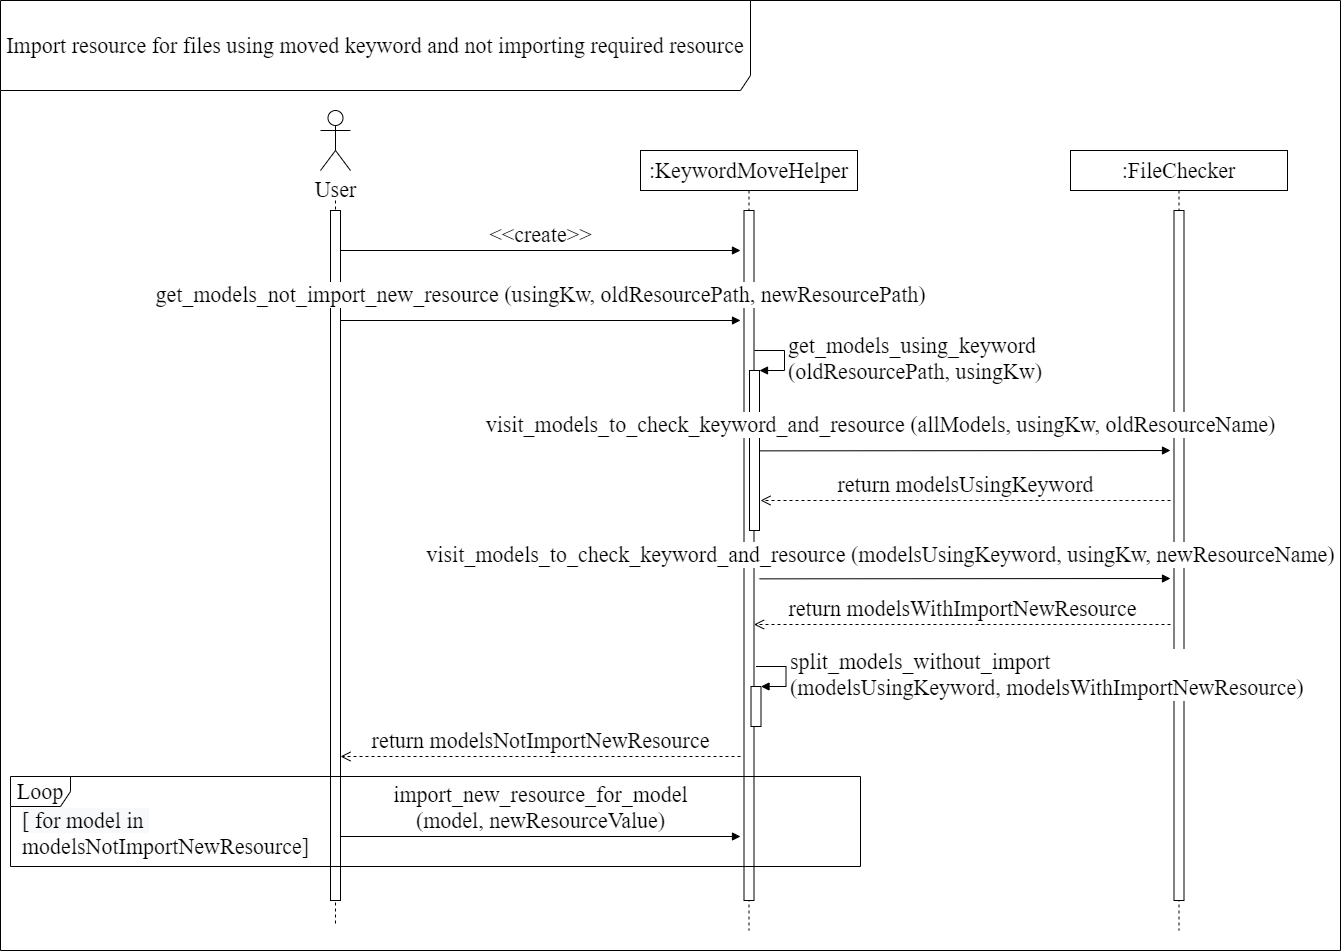
\includegraphics[width=1.0\textwidth]{picture/ch4/sequenceDiagram/Import_resource_for_files_using_moved_keyword_and_not_importing_required_resource_sequence_diagram.png}
    \caption{搜尋使用被移動關鍵字但未引入所需測試資源的測試檔案並自動引入之循序圖}
    \label{f4.8}
\end{figure}

\section{外掛程式擴充之實作}\label{s4.6}
\indent
圖\ref{f4.9}為外掛程式擴充後之類別圖,下列將介紹因擴充所新增之類別:

\begin{itemize}

\item\textbf{NewRefactorHelper:}
用於呼叫重構功能的類別。

\item\textbf{WrapStepsAsANewKeywordHandler:}
用於抽取重複步驟成為新關鍵字的handler元素,其定義WrapStepsAsANewKeywordCommand的實際行為。

\item\textbf{MoveKeywordDefinedToAnotherFileHandler:}
用於移動關鍵字宣告的handler元素,其定義MoveKeywordDefinedToAnotherFileCommand的實際行為。

\item\textbf{CreateANewKeyword:}
用於提供創立新關鍵字的使用者介面。

\item\textbf{AddArgumentsForKeywordReplacingSameSteps:}
用於提供取代重複步驟時,可新增關鍵字參數的使用者介面。

\item\textbf{FileSelectionView:}
用於顯示檔案樹狀結構及選擇檔案目標的視圖元素。

\item\textbf{SameKeywordsSelectionView:}
用於顯示重複步驟清單及選擇取代對象的視圖元素。

\item\textbf{SameStepsBlock:}
用於儲存重複步驟資訊的類別。

\item\textbf{Keyword:}
用於儲存單一關鍵字資訊的類別。

\item\textbf{Folder:}
用於儲存資料夾資訊的類別。

\item\textbf{Model:}
用於儲存AST模型資訊的類別。

\end{itemize}

\begin{figure}[H]
	\centering
    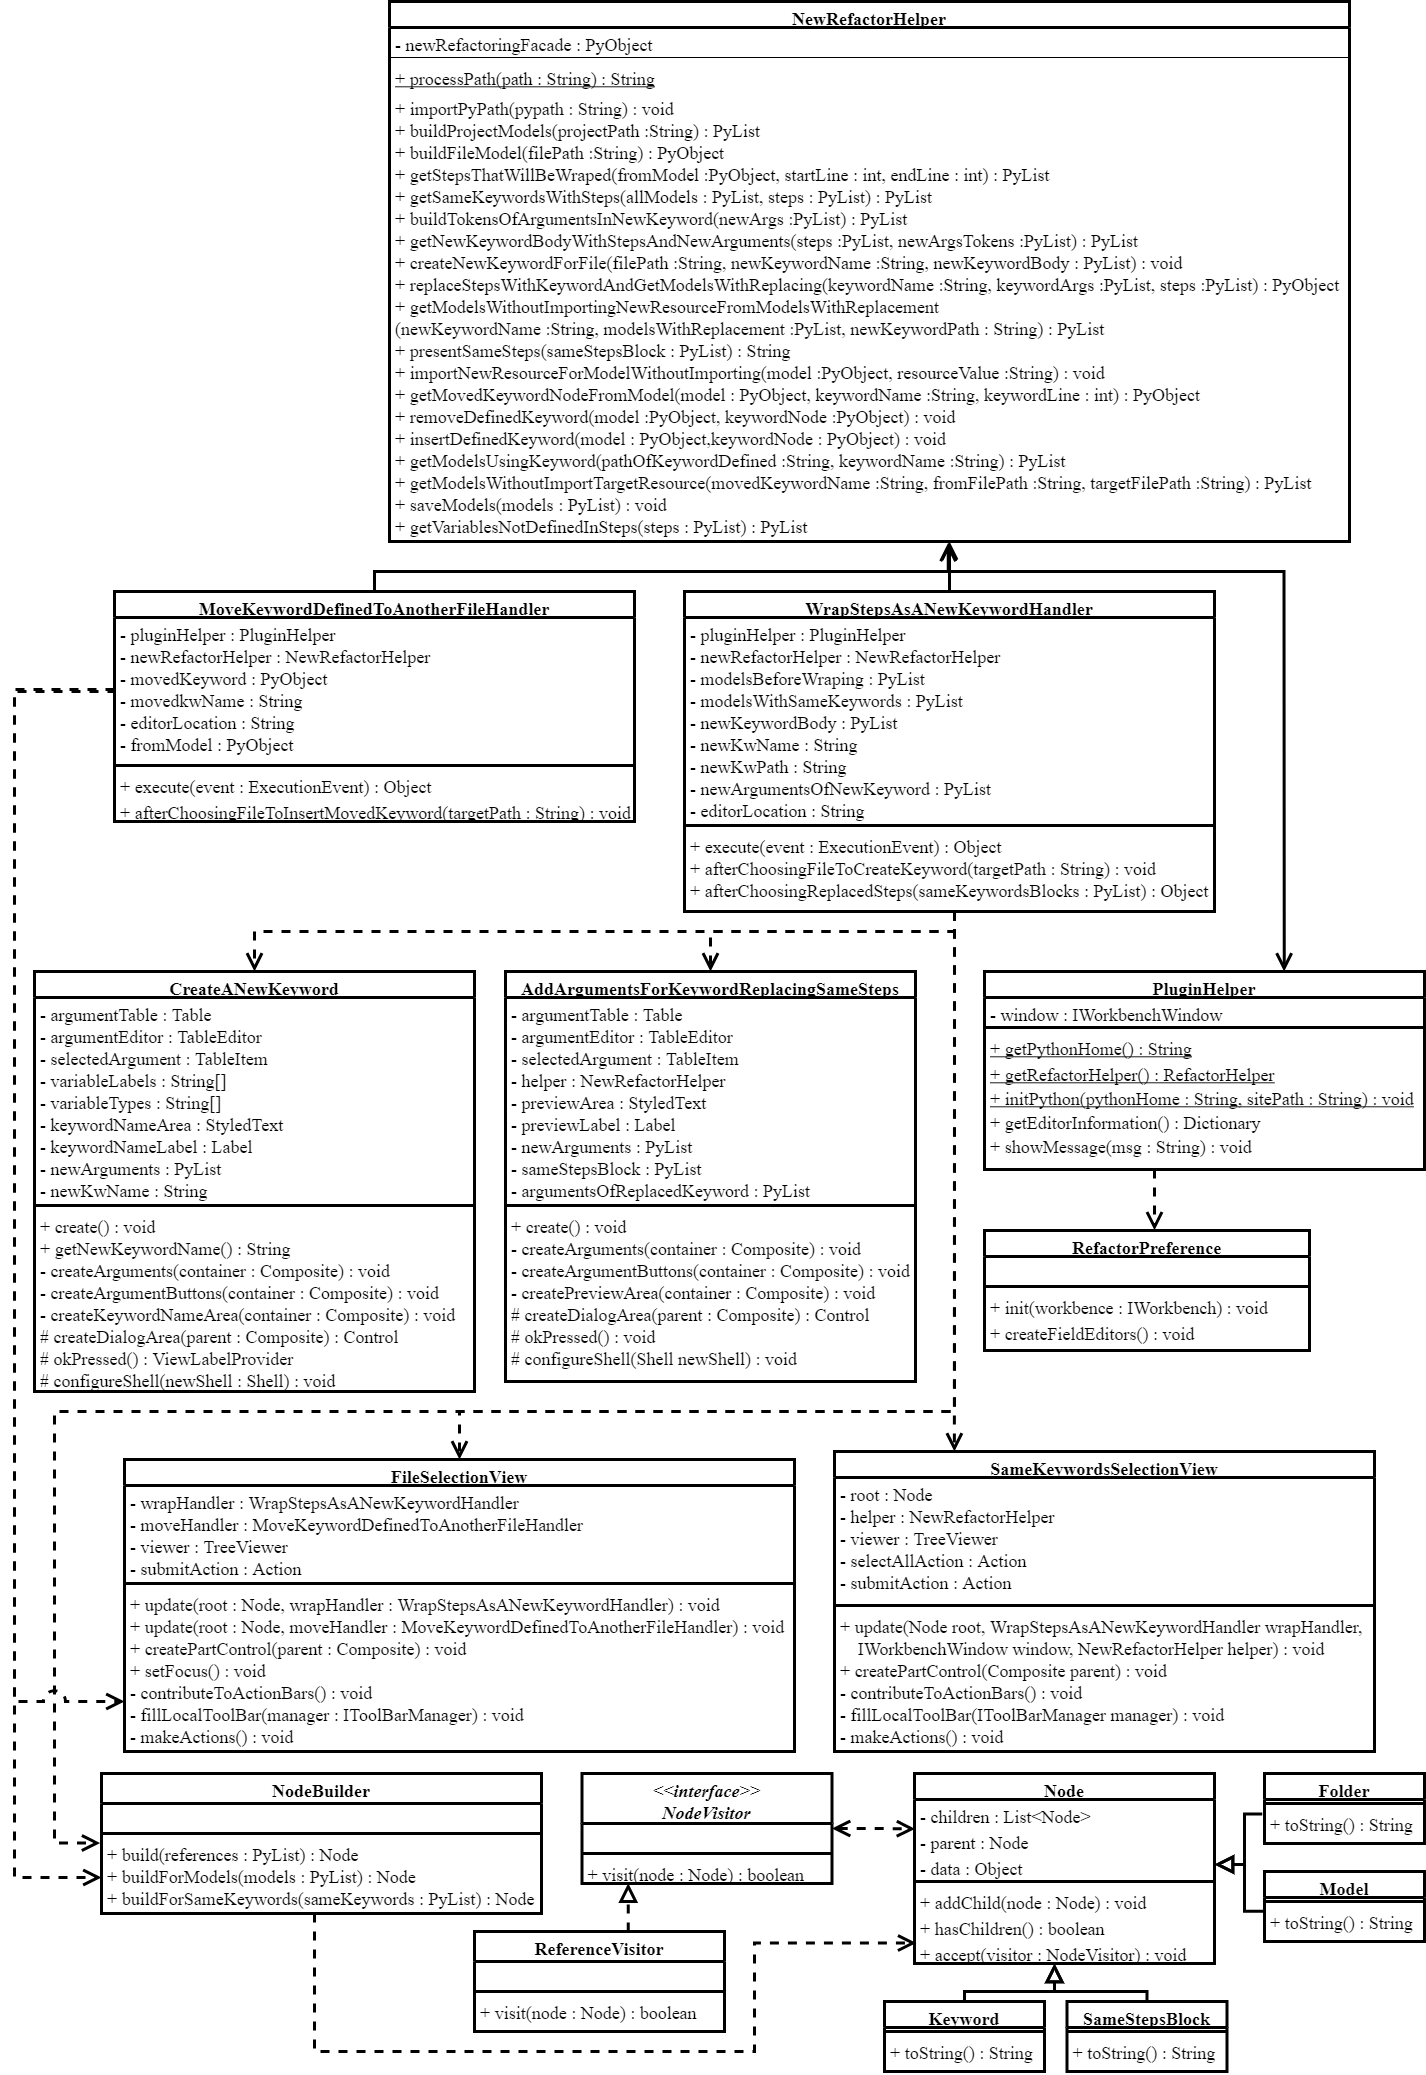
\includegraphics[width=1.0\textwidth]{picture/ch4/expanded_plugin_class_diagram.png}
    \caption{外掛程式擴充後之類別圖}
    \label{f4.9}
\end{figure}

\indent
根據\ref{s3.4}節所敘述之方法,本論文將\ref{s4.2}節所實作之重構功能與劉冠志論文\cite{LIU-Thesis}提供之Eclipse外掛程式進行結合,以此進行擴充,其中提供了抽取重複步驟為新關鍵字及移動關鍵字宣告兩種方法,下列小節將分別介紹其實作。

\subsection{抽取重複步驟成為新關鍵字}
\indent
抽取重複步驟成為新關鍵字功能提供使用者於測試腳本中抽取步驟成為新關鍵字,並搜尋重複步驟以新關鍵字進行取代,最後為其引入所需測試資源,此功能實作共可分為三部分進行講解。第一部分為抽取步驟成為新關鍵字,圖\ref{f4.10}為其循序圖,當WrapStepsAsANewKeywordCommand被執行時,Eclipse會呼叫定義其實際行為的WrapStepsAsANewKeywordHandler,WrapStepsAsANewKeywordHandler會透過PluginHelper取得使用者所選取的步驟、該檔案之路徑及該檔案所屬專案位置,並利用NewRefactorHelper解析專案路徑下的所有測試檔案提供後續使用。解析完成後其會從選取步驟中取出未宣告於步驟中的變數,並將其列入新關鍵字之參數,利用CreateANewKeyword提供使用者確認新關鍵字架構及輸入新關鍵字名稱,送出資訊後透過NodeBuilder將解析完成的測試檔案建置成樹狀結構,並顯示於FileSelectionView提供使用者選擇創立新關鍵字之位置,圖\ref{f4.11}為選擇新關鍵字位置之視圖實例。

\begin{figure}[H]
	\centering
    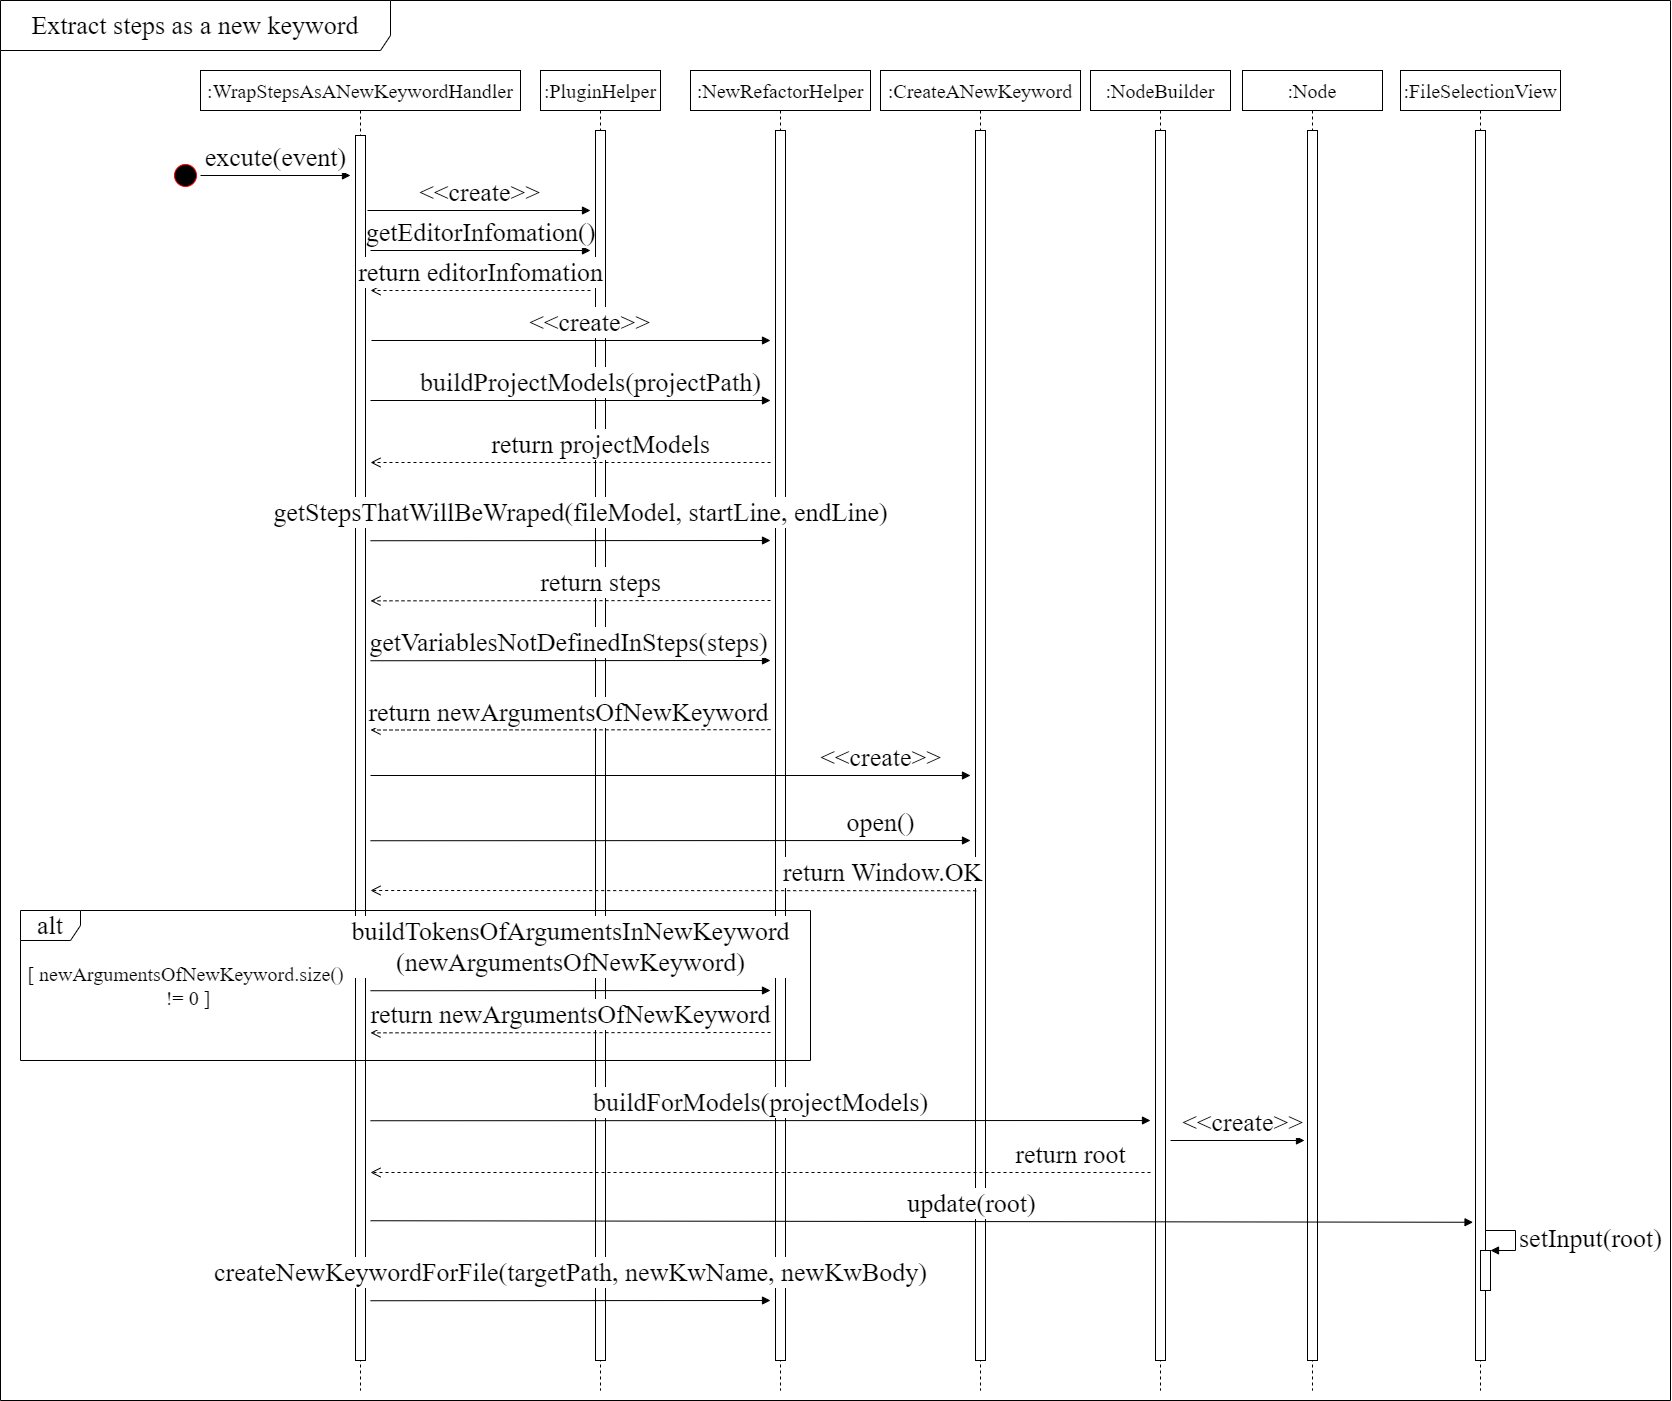
\includegraphics[width=1.05\textwidth]{picture/ch4/sequenceDiagram/wrap_steps_as_a_new_keyword_sequence_diagram.png}
    \caption{抽取步驟成為新關鍵字之循序圖}
    \label{f4.10}
\end{figure}

\begin{figure}[H]
	\centering
    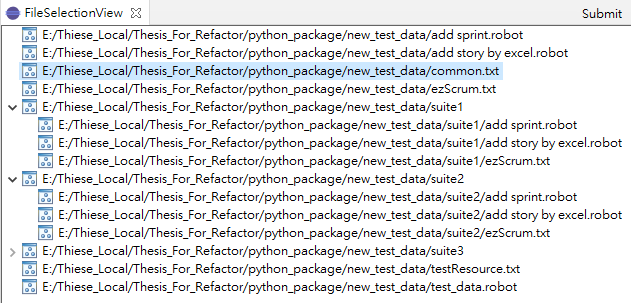
\includegraphics[width=0.7\textwidth]{picture/ch4/choose_file_view.PNG}
    \caption{選擇新關鍵字位置之視圖實例}
    \label{f4.11}
\end{figure}

\indent
第二部分為搜尋重複步驟並以新關鍵字進行取代,圖\ref{f4.12}為其循序圖,WrapStepsAsANewKeywordHandler利用NewRefactorHelper搜尋重複步驟,並透過NodeBuilder將所有重複步驟建置成樹狀結構,後續顯示於SameKeywordsSelectionView並提供使用者選擇欲取代之重複步驟,圖\ref{f4.13}為選擇欲取代之重複步驟的視圖實例。當使用者送出選取之重複步驟後,將透過AddArgumentsForKeywordReplacingSameSteps提供使用者為取代重複步驟之新關鍵字加入參數實際資料的視窗,其會顯示重複步驟內容及參數資料的輸入介面,圖\ref{f4.14}為其視窗實例。

\begin{figure}[H]
	\centering
    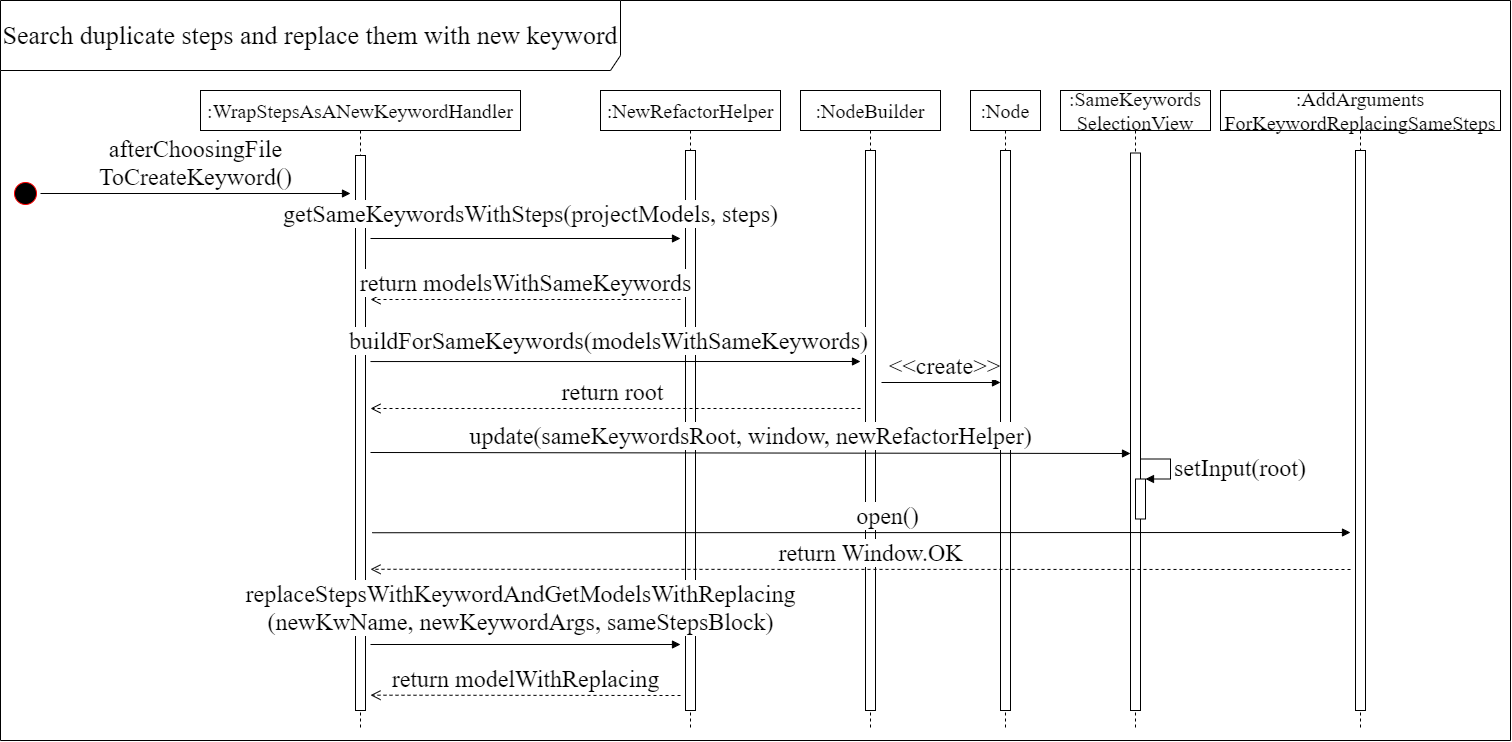
\includegraphics[width=1.0\textwidth]{picture/ch4/sequenceDiagram/Search_duplicate_steps_and_replace_sequence_diagram_in_eclipse.png}
    \caption{搜尋重複步驟並以新關鍵字進行取代之循序圖}
    \label{f4.12}
\end{figure}

\begin{figure}[H]
	\centering
    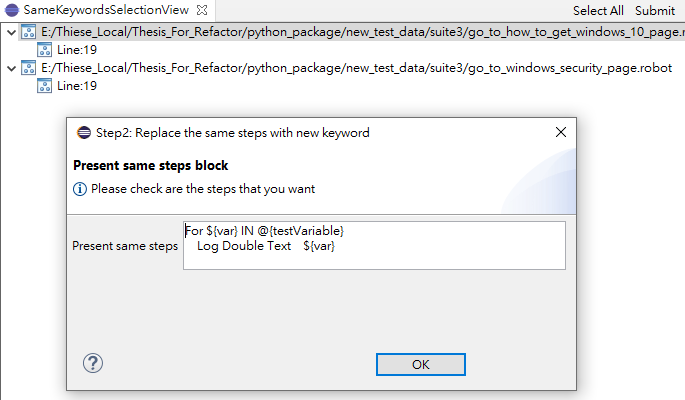
\includegraphics[width=0.6\textwidth]{picture/ch4/replace_duplicate_steps_with_new_keyword_view.PNG}
    \caption{選擇需以新關鍵字取代之重複步驟的視圖實例}
    \label{f4.13}
\end{figure}

\begin{figure}[H]
	\centering
    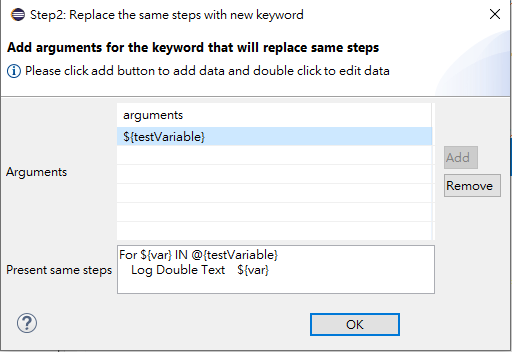
\includegraphics[width=0.5\textwidth]{picture/ch4/add_argument_for_keyword_replacing_duplicate_steps_dialog.png}
    \caption{取代重複步驟之新關鍵字加入參數實際資料之視窗實例}
    \label{f4.14}
\end{figure}

\indent
第三部分為引入新關鍵字所需之測試資源,圖\ref{f4.15}為其循序圖,透過NewRefactorHelper於使用新關鍵字之測試檔案中,搜尋未引入所需測試資源的檔案,並將所需測試資源及使用新關鍵字之檔案資訊進行路徑比對,最後為其引入所需之相對路徑。

\begin{figure}[H]
	\centering
    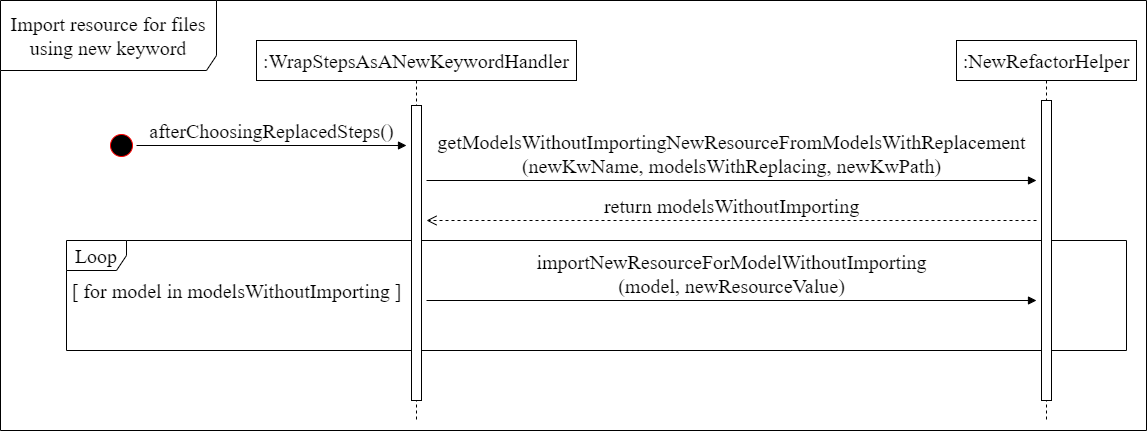
\includegraphics[width=1.0\textwidth]{picture/ch4/sequenceDiagram/Import_resource_for_new_keyword_in_eclipse_sequence_diagram.png}
    \caption{引入新關鍵字所需測試資源之循序圖}
    \label{f4.15}
\end{figure}

\subsection{移動關鍵字宣告}
%\indent
%移動關鍵字宣告提供使用者於測試檔案中移動關鍵字宣告,並於移動後自動為原先已使用此關鍵字之測試檔案引入其所需之測試資源。圖\ref{f4.16}為其循序圖,當MoveKeywordDefinedToAnotherFileCommand被執行時,Eclipse會呼叫定義其實際行為的MoveKeywordDefinedToAnotherFileHandler,其透過PluginHelper取得使用者所選取之關鍵字宣告、該檔案之路徑及該檔案所屬專案位置,並利用NewRefactorHelper解析專案路徑下的所有測試檔案提供後續使用。解析完成後其會透過NodeBuilder將解析完成的測試檔案建置成樹狀結構,並顯示於FileSelectionView提供使用者選擇關鍵字宣告所要移動的目標位置。
%
%\indent
%使用者提交目標位置後,MoveKeywordDefinedToAnotherFileHandler透過NewRefactorHelper將關鍵字宣告完整移動到目標檔案上,後續其將會於專案下的全部測試檔案中搜尋使用此關鍵字的測試檔案,並且將所需測試資源及使用此關鍵字之檔案資訊進行路徑比對,最後透過NewRefactorHelper為其引入所需測試資源之相對路徑,並於完成後更新FileSelectionView及編輯器之內容。
\indent
使用者可於測試檔案中移動關鍵字宣告,並於移動後為原先已使用此關鍵字之測試檔案引入其所需測試資源。圖\ref{f4.16}為其循序圖,當MoveKeywordDefinedToAnotherFileCommand被執行時,Eclipse會呼叫定義其實際行為的MoveKeywordDefinedToAnotherFileHandler,其透過PluginHelper取得選取之關鍵字宣告、該檔案之路徑及該檔案所屬專案位置,並利用NewRefactorHelper解析專案路徑下的所有測試檔案。透過NodeBuilder將解析完成的測試檔案建置成樹狀結構,並顯示於FileSelectionView提供使用者選擇移動的目標檔案。提交目標檔案後,透過NewRefactorHelper將關鍵字宣告移動到目標檔案上,並搜尋所有使用此關鍵字但未引入所需測試資源的測試檔案,最後為其引入所需測試資源之相對路徑。

\begin{figure}[H]
	\centering
    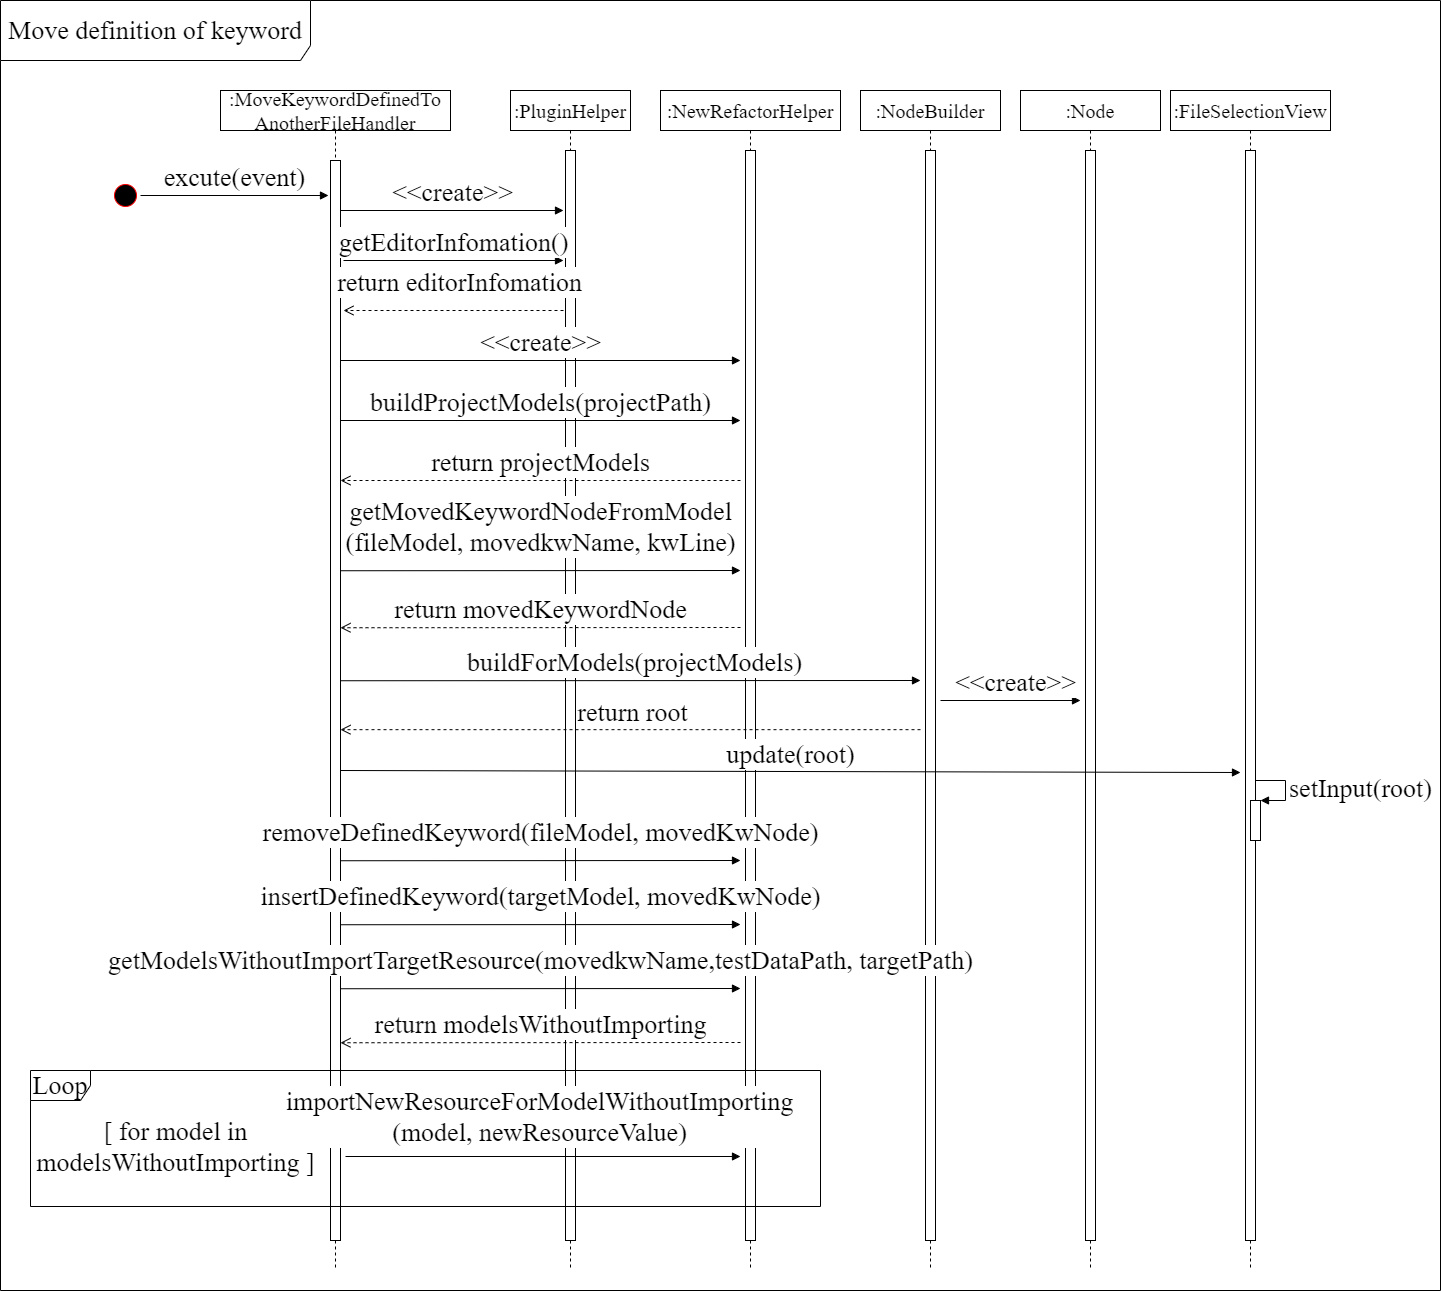
\includegraphics[width=1.0\textwidth]{picture/ch4/sequenceDiagram/Move_definition_of_keyword_in_eclipse_sequence_diagram.png}
    \caption{移動關鍵字宣告之循序圖}
    \label{f4.16}
\end{figure}